\section{Ablation Studies}
\label{app:ablation}

In this appendix, we present ablation studies examining the effect of the proposed stabilization techniques for the forward and backward pass, as well as the influence of the selected max-pooling implementation, see \cref{subsec:other_components}.

\subsection{Backward Pass Stabilization Ablation}

\renewcommand\cellalign{cc}

\begin{table*}[h!]
    \centering
    \footnotesize
    \setlength{\tabcolsep}{5pt}
    \renewcommand{\arraystretch}{1.2}

    \begin{tabular}{|c|c|c|c|c|c|c|c|}
    \noalign{\global\arrayrulewidth=1pt}
    \hline
    \noalign{\global\arrayrulewidth=0.4pt}
    \textbf{Method} & \textbf{Metric} & $\alpha \ 0.50$ & $\alpha \ 0.45$ & $\alpha \ 0.40$ & $\alpha \ 0.35$ & $\alpha \ 0.30$ & $\alpha \ 0.00$ \\
    \noalign{\global\arrayrulewidth=1pt}
    \hline
    \noalign{\global\arrayrulewidth=0.4pt}
    \multirow{4}{*}{\makecell{\textbf{SplitGrad (wta)}\\(26, g), abs}} & Point. $\uparrow$ & 0.8975 & 0.9064 & 0.9470 & \textbf{0.9558} & 0.8887 & 0.4011 \\
    \cline{2-8}
     & Attr. Loc. $\uparrow$ & 0.5434 & 0.5476 & 0.6051 & \textbf{0.6169} & 0.5346 & 0.4486 \\
    \cline{2-8}
     & Max Sens. $\downarrow$ & 0.6160 & 0.6071 & 0.4399 & 0.2382 & 0.3344 & \textbf{0.0283} \\
    \cline{2-8}
     & Pixel Fl. @20 $\uparrow$ & 1.5270 & 1.5337 & \textbf{1.5808} & 1.4476 & 1.3171 & 1.2471 \\
    \noalign{\global\arrayrulewidth=1pt}
    \hline
    \noalign{\global\arrayrulewidth=0.4pt}
    \multirow{4}{*}{\makecell{\textbf{SplitGrad}\\(26, g), abs}} & Point. $\uparrow$ & 0.8975 & 0.9064 & \textbf{0.9470} & 0.9099 & 0.2827 & 0.6413 \\
    \cline{2-8}
     & Attr. Loc. $\uparrow$ & 0.5434 & 0.5476 & \textbf{0.6037} & 0.5216 & 0.4245 & 0.4563 \\
    \cline{2-8}
     & Max Sens. $\downarrow$ & 0.6171 & 0.6102 & 0.4426 & 0.3864 & 0.0622 & \textbf{0.0079} \\
    \cline{2-8}
     & Pixel Fl. @20 $\uparrow$ & 1.5272 & 1.5333 & \textbf{1.5876} & 1.3702 & 0.2431 & 0.5755 \\
    \noalign{\global\arrayrulewidth=1pt}
    \hline
    \noalign{\global\arrayrulewidth=0.4pt}
    \multirow{4}{*}{\makecell{\textbf{SplitGrad (wta)}\\(14, g), abs}} & Point. $\uparrow$ & 0.8198 & 0.8198 & 0.8198 & \textbf{0.8322} & 0.8127 & 0.7898 \\
    \cline{2-8}
     & Attr. Loc. $\uparrow$ & \textbf{0.5403} & 0.5403 & 0.5402 & 0.5006 & 0.4936 & 0.4857 \\
    \cline{2-8}
     & Max Sens. $\downarrow$ & 0.8579 & 0.8597 & 0.8584 & 0.0875 & 0.0677 & \textbf{0.0481} \\
    \cline{2-8}
     & Pixel Fl. @20 $\uparrow$ & 2.1887 & \textbf{2.1894} & 2.1869 & 1.8740 & 1.8304 & 1.7684 \\
    \noalign{\global\arrayrulewidth=1pt}
    \hline
    \noalign{\global\arrayrulewidth=0.4pt}
    \multirow{4}{*}{\makecell{\textbf{SplitGrad}\\(14, g), abs}} & Point. $\uparrow$ & 0.8198 & \textbf{0.8198} & 0.8180 & 0.7951 & 0.8004 & 0.7968 \\
    \cline{2-8}
     & Attr. Loc. $\uparrow$ & 0.5403 & \textbf{0.5403} & 0.5330 & 0.5054 & 0.4926 & 0.4847 \\
    \cline{2-8}
     & Max Sens. $\downarrow$ & 0.8618 & 0.8584 & 0.8478 & 0.1103 & 0.0662 & \textbf{0.0301} \\
    \cline{2-8}
     & Pixel Fl. @20 $\uparrow$ & \textbf{2.1894} & 2.1891 & 2.1185 & 1.3425 & 1.2959 & 1.1927 \\
    \noalign{\global\arrayrulewidth=1pt}
    \hline
    \noalign{\global\arrayrulewidth=0.4pt}
    \multirow{4}{*}{\makecell{\textbf{SplitCAM (sc, wta)}\\(26, +, g), abs}} & Point. $\uparrow$ & 0.8675 & 0.8675 & \textbf{0.9382} & 0.9329 & 0.6131 & 0.8551 \\
    \cline{2-8}
     & Attr. Loc. $\uparrow$ & 0.5501 & 0.5535 & 0.6347 & \textbf{0.6627} & 0.4033 & 0.5133 \\
    \cline{2-8}
     & Max Sens. $\downarrow$ & 0.6906 & 0.6820 & 0.4573 & 0.2645 & 0.2511 & \textbf{0.1196} \\
    \cline{2-8}
     & Pixel Fl. @20 $\uparrow$ & 1.6067 & \textbf{1.6085} & 1.5849 & 1.4989 & 0.8534 & 1.5071 \\
    \noalign{\global\arrayrulewidth=1pt}
    \hline
    \noalign{\global\arrayrulewidth=0.4pt}
    \multirow{4}{*}{\makecell{\textbf{SplitCAM (sc)}\\(26, +, g), abs}} & Point. $\uparrow$ & 0.8940 & 0.8905 & \textbf{0.9346} & 0.6466 & 0.8251 & 0.8604 \\
    \cline{2-8}
     & Attr. Loc. $\uparrow$ & 0.5595 & 0.5636 & \textbf{0.6363} & 0.4015 & 0.4977 & 0.5114 \\
    \cline{2-8}
     & Max Sens. $\downarrow$ & 0.6738 & 0.6640 & 0.4520 & 0.3729 & 0.1102 & \textbf{0.1062} \\
    \cline{2-8}
     & Pixel Fl. @20 $\uparrow$ & 1.5902 & \textbf{1.5978} & 1.5906 & 0.9076 & 1.2784 & 1.3605 \\
    \noalign{\global\arrayrulewidth=1pt}
    \hline
    \noalign{\global\arrayrulewidth=0.4pt}
    \multirow{4}{*}{\makecell{\textbf{SplitCAM (sc, wta)}\\(14, g)}} & Point. $\uparrow$ & 0.8251 & 0.8251 & \textbf{0.8269} & 0.7880 & 0.7809 & 0.7703 \\
    \cline{2-8}
     & Attr. Loc. $\uparrow$ & 0.5363 & 0.5363 & \textbf{0.5435} & 0.5338 & 0.5286 & 0.5225 \\
    \cline{2-8}
     & Max Sens. $\downarrow$ & 1.0566 & 1.0569 & 1.0489 & \textbf{0.1620} & 0.1625 & 0.1630 \\
    \cline{2-8}
     & Pixel Fl. @20 $\uparrow$ & 2.4128 & 2.4130 & \textbf{2.4135} & 1.9014 & 1.8613 & 1.8731 \\
    \noalign{\global\arrayrulewidth=1pt}
    \hline
    \noalign{\global\arrayrulewidth=0.4pt}
    \multirow{4}{*}{\makecell{\textbf{SplitCAM (sc)}\\(14, g)}} & Point. $\uparrow$ & 0.8251 & 0.8251 & \textbf{0.8428} & 0.7756 & 0.7686 & 0.7756 \\
    \cline{2-8}
     & Attr. Loc. $\uparrow$ & 0.5363 & 0.5363 & \textbf{0.5626} & 0.5363 & 0.5271 & 0.5208 \\
    \cline{2-8}
     & Max Sens. $\downarrow$ & 1.0552 & 1.0593 & 1.0136 & 0.1629 & 0.1585 & \textbf{0.1555} \\
    \cline{2-8}
     & Pixel Fl. @20 $\uparrow$ & 2.4171 & \textbf{2.4172} & 2.4065 & 1.5032 & 1.5082 & 1.5139 \\
    \noalign{\global\arrayrulewidth=1pt}
    \hline
    \noalign{\global\arrayrulewidth=0.4pt}
    \end{tabular}

    \caption{Alpha ablation as performed in \cref{subsec:ablation} across four SplitGrad and SplitCAM configuration of layers $14$ and $26$ respectively. The notation is similar to \cref{tab:eval_vgg_main}.}
    \label{tab:alpha_comparison_by_method}
\end{table*}

In this subsection, we present the full ablation study referenced in \cref{subsec:ablation}. 
\Cref{tab:alpha_comparison_by_method} reports the $\alpha$--ablation results for SplitCAM 
and SplitGrad across selected configurations.

Overall, we observe that performance generally improves as $\alpha$ decreases below $0.5$, 
while all metrics---except Maximum Sensitivity---exhibit a sharp performance drop at 
$\alpha = 0.0$. This highlights that the stabilization mechanism in the backward pass plays 
a crucial role in the effectiveness of both methods. While the improvements in the 
Pixel~Flipping metric are modest, the gains observed in the two localization metrics and 
the robustness metric are substantial.

The table further provides pairwise comparisons between configurations using max-pooling 
in convex mode versus the ``winner-takes-it-all'' mode, see \cref{subsec:other_components}. For $\alpha$ values close to $0.5$, 
the differences across the SplitCAM and SplitGrad variants are minimal, indicating that the 
impact of max-pooling on SplitCAM's forward pass is minor in this regime. We emphasize that, 
since split-pair gradients coincide with the scaled version of the original gradients for $\alpha = 0.5$, the choice 
of max-pooling operation has no influence on the gradients in this case. The impact 
becomes most apparent for $\alpha \in \{0.30, 0.35\}$, where the ``winner-takes-it-all'' mode 
shows mostly stronger performance than the monotone mode across all methods and metrics.

\subsection{Forward Pass Stabilization Ablation}

In this subsection we want to investigate the influence of the forward stabilization procedure on SplitLRP's performance of layer configurations selected by the evaluation framework \cref{subsec:eval_framework} as well as performance of SplitCAM on manually selected layer configurations.
As a baseline, we introduce a shifting mode that effectively shifts the activations of positive neurons to half of the respective original activation and the activations of negative neurons to the negative half of it.
We also tested a SplitCAM variant with a forward pass without stabilization, where we observe an activation explosion in late VGG16 layers in the order of $10^{18}$ resulting in numerical errors in the order of $10^9$ despite trying to correct the activations in every layer such that their difference equals the original activation.
For SplitLRP, the absence of the forward stabilization produced nearly entirely white saliency maps with only small, random, and semantically meaningless artifacts. Since these results were clearly unusable, we did not compute quantitative metrics for this setting.

\subsubsection{SplitCAM}

\Cref{tab:alpha_comparison_none} summarizes the performance of all SplitCAM configurations---corresponding to those in \cref{tab:alpha_comparison_shift}---\emph{without} forward-pass stabilization.
\Cref{tab:alpha_comparison_shift} presents the results \emph{with} the shifting-based stabilization procedure.

\subsubsection{SplitLRP}

\Cref{tab:lrp_scale_shift_comparison} directly compares SplitLRP using shifting versus scaling stabilization in the forward pass.
For both layer-7 configurations, replacing scaling with shifting leads to substantial performance drops across all metrics.
For the later-layer configurations, the picture is mixed: while shifting yields slightly higher Attribution Localization scores, the scaling variants achieve markedly better Pointing Game performance and significantly improved robustness (Maximum Sensitivity).

These findings highlight the clear advantage of using scaled split-pair activations -- and not the original activations -- for LRP within the DC-decomposition framework.

\begin{longtable}{p{4.5cm}|c|cccccc}
    \caption{Scale vs Shift Comparison for SplitLRP Methods on VGG16.}
    \label{tab:lrp_scale_shift_comparison} \\
    \toprule
    \textbf{Method} & \textbf{Type} & \textbf{Select.} & \textbf{Attr. Loc.} & \textbf{Point.} & \textbf{Pixel Fl.} & \textbf{Pixel Fl.} & \textbf{Max Sens.} \\
     & & \textbf{$\downarrow$} & \textbf{$\uparrow$} & \textbf{$\uparrow$} & \textbf{AUC@5 $\uparrow$} & \textbf{AUC@20 $\uparrow$} & \textbf{$\downarrow$} \\
    \midrule
    \endfirsthead
    
    \multicolumn{8}{c}%
    {{\tablename\ \thetable{} -- continued from previous page}} \\
    \toprule
    \textbf{Method} & \textbf{Type} & \textbf{Select.} & \textbf{Attr. Loc.} & \textbf{Point.} & \textbf{Pixel Fl.} & \textbf{Pixel Fl.} & \textbf{Max Sens.} \\
     & & \textbf{$\downarrow$} & \textbf{$\uparrow$} & \textbf{$\uparrow$} & \textbf{AUC@5 $\uparrow$} & \textbf{AUC@20 $\uparrow$} & \textbf{$\downarrow$} \\
    \midrule
    \endhead
    
    \midrule
    \multicolumn{8}{r}{{Continued on next page}} \\
    \midrule
    \endfoot
    
    \bottomrule
    \endlastfoot
    
    \multirow{2}{*}{SplitLRP (wta), 7} & sc & \textbf{3.235} & \textbf{-0.036} & \textbf{0.836} & \textbf{0.296} & \textbf{2.291} & \textbf{0.866} \\
     & sh & 3.619 & -0.610 & 0.698 & 0.260 & 2.070 & 0.914 \\
    \cmidrule(lr){1-8}

    \multirow{2}{*}{SplitLRP (wta), 26, abs} & sc & \textbf{5.168} & 0.588 & 0.871 & 0.151 & 1.473 & \textbf{0.282} \\
     & sh & 5.168 & \textbf{0.628} & \textbf{0.877} & \textbf{0.161} & \textbf{1.478} & 0.468 \\
    \cmidrule(lr){1-8}

    \multirow{2}{*}{SplitLRP, 7} & sc & \textbf{3.235} & \textbf{-0.036} & \textbf{0.836} & \textbf{0.296} & \textbf{2.291} & \textbf{0.866} \\
     & sh & 3.619 & -0.695 & 0.698 & 0.260 & 2.070 & 0.914 \\
    \cmidrule(lr){1-8}

    \multirow{2}{*}{SplitLRP, 19} & sc & 5.168 & 0.588 & \textbf{0.871} & 0.151 & 1.473 & \textbf{0.282} \\
     & sh & \textbf{4.955} & \textbf{0.629} & 0.853 & \textbf{0.197} & \textbf{1.692} & 0.507 \\
    \midrule
\end{longtable}
\renewcommand\cellalign{cc}

\begin{table}[htbp]
    \centering
    \footnotesize
    \setlength{\tabcolsep}{5pt}
    \renewcommand{\arraystretch}{1.2}

    \begin{tabular}{|c|c|c|c|c|c|c|c|}
    \noalign{\global\arrayrulewidth=1pt}
    \hline
    \noalign{\global\arrayrulewidth=0.4pt}
    \textbf{Method} & \textbf{Metric} & $\alpha \ 0.50$ & $\alpha \ 0.45$ & $\alpha \ 0.40$ & $\alpha \ 0.35$ & $\alpha \ 0.30$ & $\alpha \ 0.00$ \\
    \noalign{\global\arrayrulewidth=1pt}
    \hline
    \noalign{\global\arrayrulewidth=0.4pt}
    \multirow{4}{*}{\makecell{\textbf{SplitCAM (sc, wta)}\\(26, +, g), abs}} & Point. $\uparrow$ & 0.7686 & 0.7686 & 0.8632 & \textbf{0.8712} & 0.3441 & 0.5453 \\
    \cline{2-8}
     & Attr. Loc. $\uparrow$ & 0.5374 & 0.5412 & 0.5943 & \textbf{0.6118} & 0.3595 & 0.4569 \\
    \cline{2-8}
     & Max Sens. $\downarrow$ & \cellcolor{green!20}0.6578 & \cellcolor{green!20}0.6507 & 0.4841 & 0.2873 & \cellcolor{green!20}0.1918 & \cellcolor{green!20}\textbf{0.0135} \\
    \cline{2-8}
     & Pixel Fl. @20 $\uparrow$ & 1.2744 & 1.2859 & \textbf{1.3209} & 1.1792 & 0.4430 & 0.6527 \\
    \noalign{\global\arrayrulewidth=1pt}
    \hline
    \noalign{\global\arrayrulewidth=0.4pt}
    \multirow{4}{*}{\makecell{\textbf{SplitCAM (sc)}\\(26, +, g), abs}} & Point. $\uparrow$ & 0.7565 & 0.7565 & \textbf{0.8451} & 0.3783 & 0.4507 & 0.4970 \\
    \cline{2-8}
     & Attr. Loc. $\uparrow$ & 0.5346 & 0.5384 & \textbf{0.5897} & 0.3663 & 0.4420 & 0.4545 \\
    \cline{2-8}
     & Max Sens. $\downarrow$ & \cellcolor{green!20}0.6604 & \cellcolor{green!20}0.6512 & 0.4985 & \cellcolor{green!20}0.3077 & \cellcolor{green!20}0.0279 & \cellcolor{green!20}\textbf{0.0043} \\
    \cline{2-8}
     & Pixel Fl. @20 $\uparrow$ & 1.2680 & 1.2856 & \textbf{1.3295} & 0.5912 & 0.4906 & 0.5563 \\
    \noalign{\global\arrayrulewidth=1pt}
    \hline
    \noalign{\global\arrayrulewidth=0.4pt}
    \multirow{4}{*}{\makecell{\textbf{SplitCAM (sc, wta)}\\(14, g)}} & Point. $\uparrow$ & \cellcolor{green!20}\textbf{0.8491} & \cellcolor{green!20}0.8491 & \cellcolor{green!20}0.8491 & 0.7867 & \cellcolor{green!20}0.7847 & 0.7686 \\
    \cline{2-8}
     & Attr. Loc. $\uparrow$ & 0.5324 & 0.5321 & \textbf{0.5406} & 0.5306 & 0.5261 & 0.5200 \\
    \cline{2-8}
     & Max Sens. $\downarrow$ & 1.0834 & 1.0814 & 1.0885 & \textbf{0.2271} & 0.2309 & 0.2384 \\
    \cline{2-8}
     & Pixel Fl. @20 $\uparrow$ & \cellcolor{green!20}2.4454 & \cellcolor{green!20}2.4482 & \cellcolor{green!20}\textbf{2.4486} & \cellcolor{green!20}1.9588 & \cellcolor{green!20}1.9193 & \cellcolor{green!20}1.9349 \\
    \noalign{\global\arrayrulewidth=1pt}
    \hline
    \noalign{\global\arrayrulewidth=0.4pt}
    \multirow{4}{*}{\makecell{\textbf{SplitCAM (sc)}\\(14, g)}} & Point. $\uparrow$ & 0.7746 & 0.7767 & \textbf{0.7847} & 0.5855 & 0.5594 & 0.5573 \\
    \cline{2-8}
     & Attr. Loc. $\uparrow$ & 0.4003 & 0.4144 & \textbf{0.5517} & 0.5300 & 0.5209 & 0.5137 \\
    \cline{2-8}
     & Max Sens. $\downarrow$ & 1.5733 & 1.5627 & 1.5443 & \textbf{1.2661} & 1.3939 & 1.4272 \\
    \cline{2-8}
     & Pixel Fl. @20 $\uparrow$ & 2.1298 & \textbf{2.1384} & 2.1371 & \cellcolor{green!20}1.6669 & \cellcolor{green!20}1.6793 & \cellcolor{green!20}1.6740 \\
    \noalign{\global\arrayrulewidth=1pt}
    \hline
    \noalign{\global\arrayrulewidth=0.4pt}
    \end{tabular}

    \caption{Alpha ablation for scale normalization across four SplitCAM configurations of layers 14 and 26. Here, in the forward pass no stabilization is applied. Notation and structure is similar to \cref{tab:alpha_comparison_by_method}. Green cells indicate better performance of the method compared to the default variant with scale stabilization in the forward pass.}
    \label{tab:alpha_comparison_none}
\end{table}
\renewcommand\cellalign{cc}

\begin{table}[htbp]
    \centering
    \footnotesize
    \setlength{\tabcolsep}{5pt}
    \renewcommand{\arraystretch}{1.2}

    \begin{tabular}{|c|c|c|c|c|c|c|c|}
    \noalign{\global\arrayrulewidth=1pt}
    \hline
    \noalign{\global\arrayrulewidth=0.4pt}
    \textbf{Method} & \textbf{Metric} & $\alpha \ 0.50$ & $\alpha \ 0.45$ & $\alpha \ 0.40$ & $\alpha \ 0.35$ & $\alpha \ 0.30$ & $\alpha \ 0.00$ \\
    \noalign{\global\arrayrulewidth=1pt}
    \hline
    \noalign{\global\arrayrulewidth=0.4pt}
    \multirow{4}{*}{\makecell{\textbf{SplitCAM (sc, wta)}\\(26, +, g), abs}} & Point. $\uparrow$ & 0.8330 & 0.8149 & 0.7968 & \textbf{0.9235} & 0.6036 & \cellcolor{green!20}0.8592 \\
    \cline{2-8}
     & Attr. Loc. $\uparrow$ & 0.5242 & 0.5203 & 0.5147 & \textbf{0.6549} & 0.3968 & 0.5093 \\
    \cline{2-8}
     & Max Sens. $\downarrow$ & \cellcolor{green!20}0.6180 & \cellcolor{green!20}0.6182 & 0.6509 & 0.3104 & 0.2791 & \textbf{0.1665} \\
    \cline{2-8}
     & Pixel Fl. @20 $\uparrow$ & \cellcolor{green!20}\textbf{1.6804} & \cellcolor{green!20}1.6646 & 1.5065 & 1.4962 & \cellcolor{green!20}0.8896 & \cellcolor{green!20}1.5405 \\
    \noalign{\global\arrayrulewidth=1pt}
    \hline
    \noalign{\global\arrayrulewidth=0.4pt}
    \multirow{4}{*}{\makecell{\textbf{SplitCAM (sc)}\\(26, +, g), abs}} & Point. $\uparrow$ & 0.8330 & 0.8149 & 0.7988 & 0.5654 & \cellcolor{green!20}0.8431 & \cellcolor{green!20}\textbf{0.8652} \\
    \cline{2-8}
     & Attr. Loc. $\uparrow$ & \textbf{0.5242} & 0.5203 & 0.5076 & 0.3736 & 0.4949 & 0.5094 \\
    \cline{2-8}
     & Max Sens. $\downarrow$ & \cellcolor{green!20}0.6129 & \cellcolor{green!20}0.6168 & 0.6494 & 0.3820 & 0.1686 & \textbf{0.1664} \\
    \cline{2-8}
     & Pixel Fl. @20 $\uparrow$ & \cellcolor{green!20}\textbf{1.6804} & \cellcolor{green!20}1.6646 & 1.5105 & 0.8714 & \cellcolor{green!20}1.4289 & \cellcolor{green!20}1.4765 \\
    \noalign{\global\arrayrulewidth=1pt}
    \hline
    \noalign{\global\arrayrulewidth=0.4pt}
    \multirow{4}{*}{\makecell{\textbf{SplitCAM (sc, wta)}\\(14, g)}} & Point. $\uparrow$ & \cellcolor{green!20}\textbf{0.8310} & \cellcolor{green!20}0.8310 & \cellcolor{green!20}0.8310 & \cellcolor{green!20}0.7887 & \cellcolor{green!20}0.7827 & \cellcolor{green!20}0.7726 \\
    \cline{2-8}
     & Attr. Loc. $\uparrow$ & 0.5312 & 0.5312 & \textbf{0.5376} & 0.5315 & 0.5264 & 0.5203 \\
    \cline{2-8}
     & Max Sens. $\downarrow$ & \cellcolor{green!20}1.0562 & \cellcolor{green!20}1.0521 & 1.0649 & \textbf{0.1633} & 0.1641 & 0.1642 \\
    \cline{2-8}
     & Pixel Fl. @20 $\uparrow$ & \cellcolor{green!20}\textbf{2.4412} & \cellcolor{green!20}2.4412 & \cellcolor{green!20}2.4400 & \cellcolor{green!20}1.9306 & \cellcolor{green!20}1.8953 & \cellcolor{green!20}1.9059 \\
    \noalign{\global\arrayrulewidth=1pt}
    \hline
    \noalign{\global\arrayrulewidth=0.4pt}
    \multirow{4}{*}{\makecell{\textbf{SplitCAM (sc)}\\(14, g)}} & Point. $\uparrow$ & \cellcolor{green!20}0.8310 & \cellcolor{green!20}0.8310 & \cellcolor{green!20}\textbf{0.8431} & 0.7746 & \cellcolor{green!20}0.7706 & \cellcolor{green!20}0.7807 \\
    \cline{2-8}
     & Attr. Loc. $\uparrow$ & 0.5311 & 0.5312 & \textbf{0.5580} & 0.5337 & 0.5245 & 0.5183 \\
    \cline{2-8}
     & Max Sens. $\downarrow$ & 1.0554 & \cellcolor{green!20}1.0568 & 1.0198 & 0.1641 & 0.1587 & \textbf{0.1570} \\
    \cline{2-8}
     & Pixel Fl. @20 $\uparrow$ & \cellcolor{green!20}\textbf{2.4412} & \cellcolor{green!20}2.4411 & \cellcolor{green!20}2.4318 & \cellcolor{green!20}1.5187 & \cellcolor{green!20}1.5222 & \cellcolor{green!20}1.5329 \\
    \noalign{\global\arrayrulewidth=1pt}
    \hline
    \noalign{\global\arrayrulewidth=0.4pt}
    \end{tabular}

    \caption{Alpha ablation for scaling normalization across four SplitCAM configurations of layers 14 and 26. Here, in the forward pass we apply shift normalization. Notation and structure is similar to \cref{tab:alpha_comparison_by_method}. Green cells indicate better performance of the method compared to the default variant with scale stabilization in the forward pass.}
    \label{tab:alpha_comparison_shift}
\end{table}

\subsection{Layer Dependence Analysis}

Figure~\ref{fig:layer_dependence} shows the layer dependence of different attribution methods.
Each method is normalized independently to visualize the relative performance across different layers. Unlike the ablations of the previous section, here we only evaluated across the custom validation subset of ImageNet-S.

Overall, the plots reveal a strong layer dependence of all considered methods and metrics.
Surprisingly, the $\gamma$-LRP does not show the strongest performance in the first layer.
There are clear patterns for each of the metrics, valid across different methods.
Pixel Flipping performs exceptionally well in layer 14 across almost all methods, except SplitCAM and SplitGrad with $\alpha=0.3$.
Maximum sensitivity performs best in later layers, while exploding in the last layers for LRP and SplitGrad with $\alpha=0.3$.

\begin{figure}[htbp]
\centering
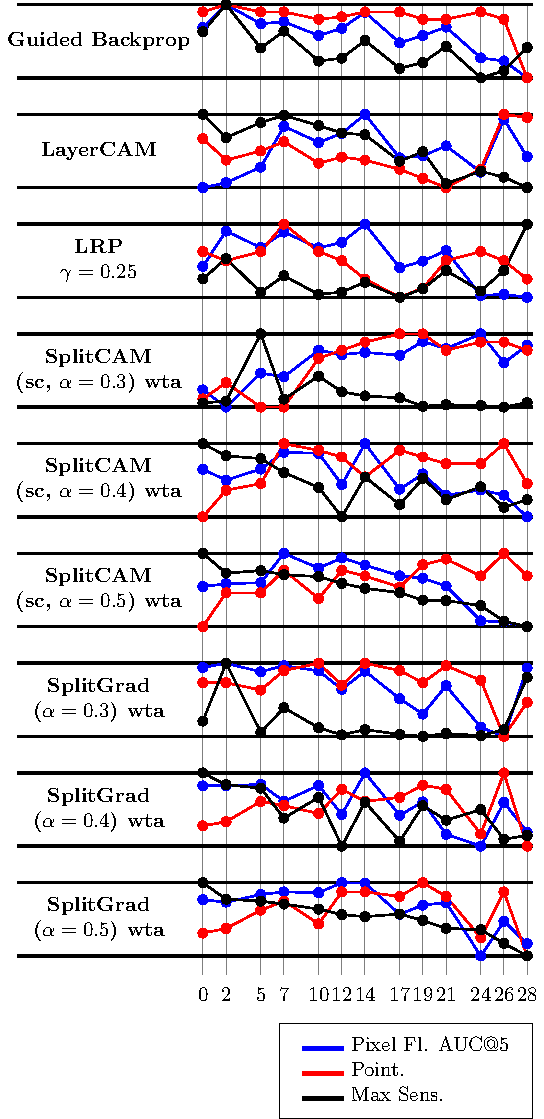
\includegraphics[width=0.5\textwidth]{figures/layer_dependence_all.pdf}
\caption{Layer dependence for different attribution methods. Each method is normalized independently to show relative performance across layers.}
\label{fig:layer_dependence}
\end{figure}

Figure~\ref{fig:layer_dependence} resembles a characteristic fingerprint of a trained classification model.
It reveals which layers localize most accurately, which exhibit the highest robustness to small input perturbations, and which activation or gradient pathways most strongly influence the Pixel Flipping behavior.
These layer-wise patterns may provide insights into how evidence is processed throughout the network and could potentially guide future diagnostics or architectural analysis.
However, a deeper investigation of these research questions lies beyond the scope of this work.